\documentclass[12pt,a4paper]{article}
\usepackage{amsmath}
\usepackage{amsfonts}
\usepackage{amssymb}
\usepackage{graphicx}
\begin{document}

\section{splines caclulations}
Splines data points are calculated at fixed energies. The energy points are uniformly distributed in logarithmic range.
The number of points and logarithmic limits are defined in \textit{constants.h}.
The number of points is \textit{max\_datapoints}, log limits are \textit{logEmin} and \textit{logEmax}.


The energy points are stored in \textit{EnergyTable} class and precalculated values are stored in \textit{energy\_table} variable.
the double array can be accessed as energy\_table.values.

The integration is done using GSL numerical integration library.

\subsection{range spline precision}
The range spline precision is checked via calculating dE/dx from inverse derivative of range spline and compared to directly calculated dE/dx.

\begin{figure}[h]
	\centering
    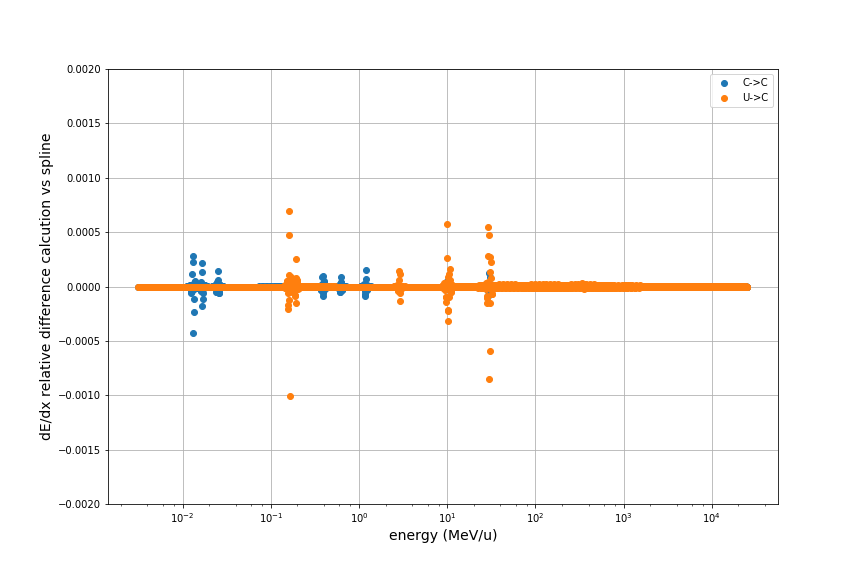
\includegraphics[width=6.5cm]{plots/dedx_difs_n500.png}
   	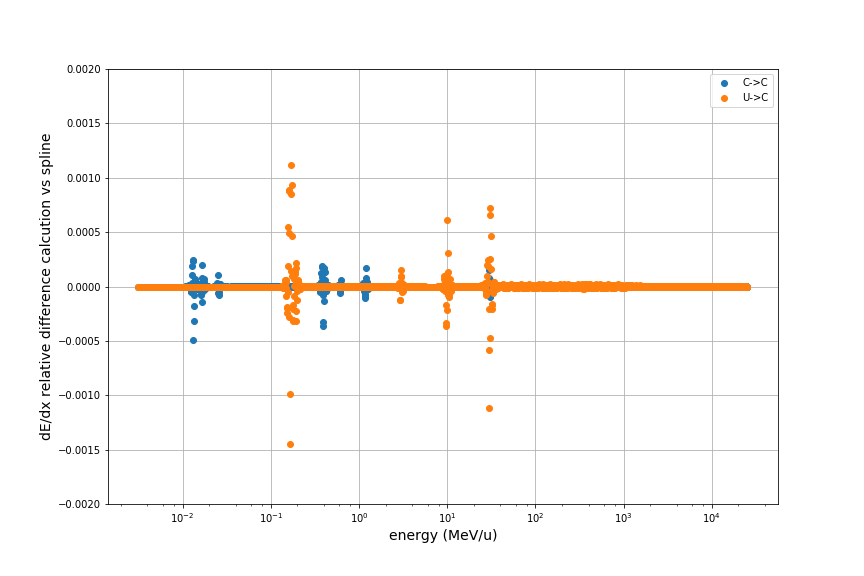
\includegraphics[width=6.5cm]{plots/dedx_difs_n400.png}
   	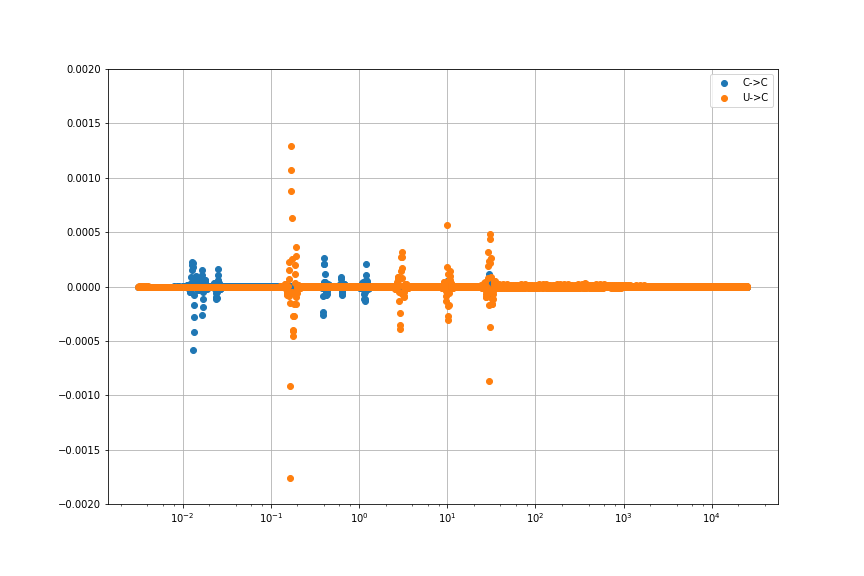
\includegraphics[width=6.5cm]{plots/dedx_difs_n300.png}
   	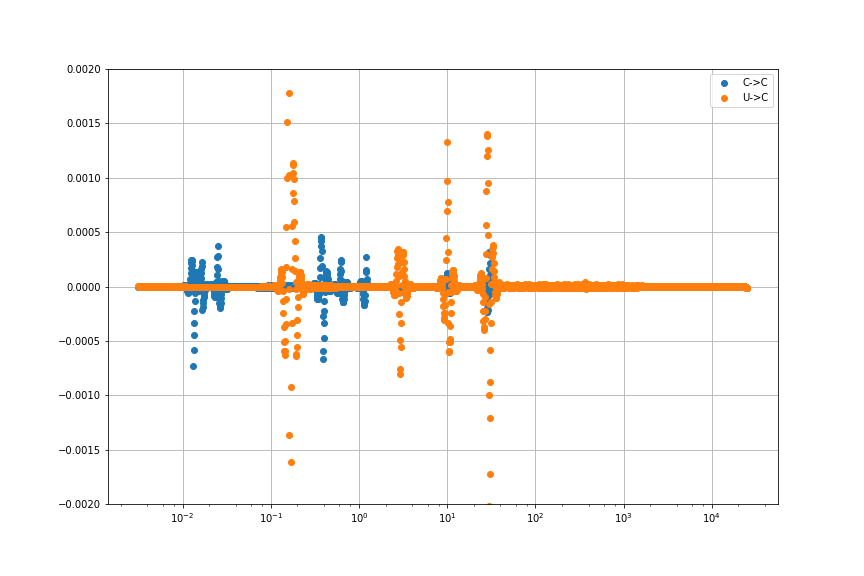
\includegraphics[width=6.5cm]{plots/dedx_difs_n200.png}
	\caption{Relative difference of dE/dx calculated directly and from range spline, number of range spline datapoints = 500(top left), 400(top right), 300(bottom left), 200(bottom right)}
\end{figure}	



\section{Benchmarks}
\subsection{Thin Target Approximation}
test: projectile: 238U@700MeV/u - 30GeV/u, material: C(1mg/cm2), 30000 calculation in loop.

reults: with thin target pproximation: 2.4s, without: 2.4s
	
\end{document}